\startchapter{Evaluation of The Gem Cutter Environment}
\label{chapter:Exp}

\begin{flushright}
\textit{...a scientist must also be absolutely like a child.  If he sees a thing, he must say that he sees it, whether it was what he thought he was going to see or not.  See first, think later, then test.  But always see first.  Otherwise you will only see what you were expecting.}
\\
Douglas Adams \cite{Adams84} \\
\end{flushright}

\section{Applying the Cognitive Dimensions Framework to the Gem Cutter}

In this section we shall apply the Cognitive Dimensions framework developed by Green to the Gem Cutter VPE.

\subsection{Abstraction Gradient}

As described in \sref{cgframeoutline} the Abstraction Gradient dimension tries to measure how much needs to be constructed
and learned in order to begin making the programming environment perform a task, and additionally how easy is it to add new abstractions to the environment.

\subsubsection{Discussion of Dimension}

In regards to the Gem Cutter, much like the VFPE, as a functional language there is a relatively small set of constructs to master before making the environment perform a task.  As a base minimum, one only needs to be familiar with the notion of a function, and how a gem is a visual representation of that concept, along with the mechanics of how to connect gems together on the tabletop.  As one wishes to do more sophisticated tasks, introduction of the additional gem types\footnote{Such as collector/emitter pairs, value gems, code gems, and record gems} will be required, however, this is still a relatively low minimum level of abstraction.  This is a great strength of the Gem Cutter, particularly from the perspective of a student learning to program, as little needs to be learned and mastered before beginning to make the environment perform basic tasks.

The Gem Cutter like most programming languages, would be an example of an abstraction-tolerant language, though only barely.  The only mechanism for introducing new abstractions is the ability to define new gems and use those gems in other gem designs.  Aside from this basic abstraction mechanic there is little or no support for introducing new abstractions.  In particular the lack of ability to introduce new types as discussed in \sref{sec:gemCutterShortcomings} greatly hinders ones ability to introduce new abstractions to reduce the complexity of larger problems.  This is mitigated somewhat by the introduction of code gems which allow one to introduce CAL code snippets at any point into a gem design.  Since CAL is very much an abstraction-tolerant language fully supporting the ability to introduce and define new types, this allows a ``loophole'' where one can bring all the expressive power of CAL to the Gem Cutter.  However, code gems will only be useful to those who already understand the CAL language.  This would be roughly analogous to requiring users of Alice to write Java code to create new object types to use in their Alice programs, which would seem rather cumbersome.

\subsubsection{Remedies, Workarounds, And Trade-offs}

Green suggests that a possible remedy for problems related to the abstraction gradient of an environment is to introduce incremental abstractions.  This would be where the environment has a low starting abstraction barrier (ie - start with a low minimum level of abstraction where little needs to be learned to begin working with the environment), and to allow the introduction of new abstractions that will aid users later.  To a certain degree the Gem Cutter does this already, as there is a relatively low minimum level of abstraction as mentioned above, and one can learn about the other gem types as they progress with the environment.  What is missing are enhanced facilities for newer abstractions, most notably in regards to types.  The introduction of a mechanism for defining a new type in a visual way would help to alleviate this aspect much more than the current ``workaround'' of using code gems.

%------------------------------------------------------------------------------------------------

\subsection{Closeness of Mapping}

As described in \sref{cgframeoutline} the dimension of Closeness of Mapping tries to measure the gap between the problem domain and the program domain. 

\subsubsection{Discussion of Dimension}

In terms of ``programming games'', the Gem Cutter imposes relatively few upon the user.  As a visual functional language, the notation of the Gem Cutter is rather concise.  Sometimes gem designs can become ``cluttered'' with an excessive number of visual entities, but this is more of an issue related to Diffuseness than of Closeness of Mapping.

Additionally, there are two other issues to consider from the perspective of Closeness of Mapping.  The first is the issue of the language's standard library support, and the second is what constructs the language allows to be built to improve the Closeness of Mapping.

With respect to the Gem Cutter, there is an extensive set of predefined gems provided to the user.  In particular, there is a great deal of library support in the Quark framework, CAL and the Gem Cutter for working with relational databases.  The DatabaseMetadata, Sql, SqlBuilder, and SqlParser modules are all imported by default into the Gem Cutter, and provide extensive support to close the gap between a problem in the domain of relational databases and the Gem Cutter environment itself.  In addition to these modules, the CAL language itself has a significant collection of modules for working in a variety of domains, any of which can be imported into the Gem Cutter.  The library support in the OpenQuark framework is not as robust as some more ``industry-proven'' languages (such as Sun's Java API), but is much more comprehensive and varied than the Prograph or VFPE environments.  

In terms of constructs to improve the Closeness of Mapping, much like the VFPE, the Gem Cutter can use higher-order functions to enable various programming ``idioms'' which can help greatly with changing the mapping from problem to program domain.

\subsubsection{Remedies, Workarounds, And Trade-offs}

There are no specific issues identified with the Gem Cutter with respect to Closeness of Mapping.  Short of additional library support, there is little that can be introduced to the Gem Cutter to improve this dimension.

%------------------------------------------------------------------------------------------------

\subsection{Consistency}

As described in \sref{cgframeoutline} the dimension of Consistency tries to address how easy is it to infer the remaining parts of the language, once one has learned part of the language.

\subsubsection{Discussion of Dimension}

As noted in \sref{sec:prevAppCG}, visual languages tend to be very consistent due to the much simpler syntax.  The Gem Cutter is no different in this respect.  In particular, once one masters the metaphor of ``gem as function'' with inputs connecting to the left side of the gem, and the single output leaving the right side, the rest of the environment becomes very easy to learn as all gems follow this pattern.

Additionally, another issue related to consistency is library regularity.  Much like the Haskell language which inspired it, CAL (and as a result the Gem Cutter) keeps argument ordering very consistent.  For example, if a gem takes two arguments, one a function and the other a primitive type (such as an Integer), then the function argument will be the first (top-most) argument in the gem display.  This follows the common functional programming convention of having higher order functions come before primitive types in argument lists.  However, one very interesting thing to note however is that while this convention is followed, there is no restriction in the Gem Cutter in terms of in what order arguments are bound.  For example, consider the \code{map()} function common to virtually all functional programming languages.  The \code{map()} function is a function which takes two arguments, a function \code{f()}, and a list of items (\(x,x_0,x_1,...,x_n\)).  The result returned is the list with the function applied to each element or the list (\(f(x),f(x_0),f(x_1),...,f(x_n)\)).

In traditional textual functional languages such as Haskell or SML, one must bind the function argument before one binds the list argument.  The consequence of this is that we can use \code{map()} to create new functions of one argument -- a list.  We cannot however use \code{map()} to create a new function of single function argument.  In the Gem Cutter, because we can bind arguments in any order, we do not have this limitation.  This would seem to be the best of both worlds, we have the flexibility and freedom to bind arguments in whichever order (thus allowing us greater expressivity), but we also have the consistency of argument ordering (though top down instead of left to right).

\subsubsection{Remedies, Workarounds, And Trade-offs}

The Gem Cutter is remarkably consistent, and as such there are no specific issues or ways that this dimension could be improved.

%------------------------------------------------------------------------------------------------

\subsection{Diffuseness}
\label{sec:eval:diffuseness}

As described in \sref{cgframeoutline} the dimension of Diffuseness (or terseness) tries to measure how many symbols are required to express a given meaning in the notation being examined.

\subsubsection{Discussion of Dimension}

With respect to the Gem Cutter, it is worth noting that the sample implementation by Green of the rocket trajectory program written in BASIC (seen in \pref{prog:basicRocket1}) was done in an iterative style, and since the Gem Cutter is a functional language there are no mechanisms for iteration instead requiring recursion to be used.  Thus while the implementation in Gem Cutter of the rocket trajectory program is based upon the BASIC version it is structured significantly differently.  Instead of having a single routine that encompasses the entire problem, we created a gem called \code{rocket1()} which given the current state of the rocket\footnote{The vertical distance, vertical velocity, horizontal distance, horizontal velocity, and current mass} at time $t$, calculates the new state of the rocket at time $t + 1$ and returns this as a 6-tuple.  In some respects, this is a solution to the rocket trajectory problem by itself.  However, to more closely match the semantics of the BASIC version, a second gem was created called \code{rocketTester()} which generates the state of the rocket from time 0 to whatever time the rocket's vertical distance becomes negative.  Presumably, Kelso had to do something similar for the implementation in the VFPE of the rocket trajectory problem, however, the layout of his implementation was not supplied so we do not know how closely his approach matched that of the Gem Cutter implementation.

\begin{program}
\begin{verbatim}
Mass = 10000
Fuel = 50
Force = 400000
Gravity = 32
WHILE Vdist >= 0
      IF Tim = 11 THEN Angle = .3941
      IF Tim > 100 THEN Force = 0 ELSE Mass = Mass - Fuel
      Vaccel = Force*COS(Angle)/Mass - Gravity
      Vveloc = Vveloc + Vaccel
      Vdist = Vdist + Vveloc
      Haccel = Force*SIN(Angle)/Mass
      Hveloc = Hveloc + Haccel
      Hdist = Hdist + Hveloc
      PRINT Tim, Vdist, Hdist
      Tim = Tim + 1
WEND
STOP
\end{verbatim}
\caption{The Implementation of the Rocket Trajectory Problem in BASIC\cite{green96}}
\label{prog:basicRocket1}
\end{program}

The breakdown of graphic entities in the two gems can be seen in \tref{tab:GCrocket1}.  The complete solution of both gems for the rocket trajectory problem required 161 different graphic entities, far more than the 131 for Prograph, 104 for LabVIEW, and 98 for the VFPE.  Note that connector lines were included in the totals for the Gem Cutter implementation.  This was different than the totals for the VFPE where connectors were not included in the total due to the fact that connection lines were not established by the user.  Connection lines were included in the total for Prograph, however, this was due to the fact that when one wishes to move a component in a Prograph layout, they also need to manually adjust the connections.  In Gem Cutter, while the connections between gems need to be established by the user, once they are established movement of gems around the tabletop does will cause the connections to be redrawn automatically.  If we leave out the connections, then the total for the Gem Cutter implementation falls to 88 graphic entities, easily the most terse of the four considered.

\begin{table}
	\caption{The Breakdown of Graphic Entities in the Gem Cutter Solution to the Rocket Trajectory Problem}
\begin{tabular}{|l|m{2.5cm}|m{3.5cm}||m{3cm}|}
\hline
\textbf{Gem Type} & \textbf{\code{rocket1()} Count} & \textbf{\code{rocketTester()} Count} & \textbf{Total For Both} \\
\hline
Connectors & 59 & 14 & 73 \\
Emitter Gems & 27 & 1 & 28 \\
Function Gems & 19 & 5 & 24 \\
Value Gems & 9 & 7 & 16 \\
Collector Gems & 12 & 1 & 13 \\
Record Selection Gems & 6 & 1 & 7 \\
\hline \hline
\textbf{Totals} & 132 & 29 & \underline{161} \\
\hline
\end{tabular}
	\label{tab:GCrocket1}
\end{table}

Also note that the single target gem was not counted in these numbers as it is a graphic entity that always appears in any gem design (it is not added by the user).  Given that there is only a single target gem for any gem design, the inclusion or exclusion of this entity will not significantly alter the graphic count either way.

The use of record selection gems to parse a tuple into subsequent parts incurs a significant number of entities as well.  While the count in \tref{tab:GCrocket1} does not seem to indicate this (as there are only 7 record selection gems), what is missing from this total is the fact that connected to the record selection gems are two connectors, and a collector and emitter pair for each (an emitter for the tuple being parsed, and a collector to ``name'' the parsed value).  Thus breaking the 6-tuple rocket state into six separate values in \code{rocket1()} adds a total of 30 entities (including connectors, 18 if we omit connectors).

In terms of screen space, the implementation of the \code{rocket1()} gem would not fit on a single 1280x960 resolution screen, instead scrolling roughly halfway past the end of the screen.  The \code{rocketTester()} gem however fit easily on a single screen, and can be seen in \fref{gcRocketTester1}.

\insertFigure{4}{gcRocketTester1}{The \code{rocketTester()} Gem}

Additionally, simple mathematical expressions tend to take up a disproportionate amount of space on the screen.  It is a much more compact representation to have a single character such as `*' to denote multiplication, than a full gem with the word ``multiply'' written on it.  One can alleviate this with code gems, however the use of code gems are not in the ``spirit'' of the visual paradigm.

Conditionals can also introduce seemingly redundant entities.  Consider the if/else statement in \pref{prog:javaIf} written in Java.  This fragment contains a single if statement, and assigns values to two different variables depending on the value of someBooleanExpression.  This same fragment translated into Gem Cutter would be what we see in \fref{gcIfStatement}.  Note that there are now two if statements, one to determine the value of \code{var1}, and another to determine the value of \code{var2}.  As there is no mechanism for ``blocks'' of code in the Gem Cutter, one has to separate the two collections of statements into separate if statements.

\begin{program}
\begin{verbatim}
if (someBooleanExpression)
{
	var1 = 10;
	var2 = 20;
}
else
{
	var1 = 20;
	var2 = 10;
}
\end{verbatim}
\caption{A Hypothetical if Statement in Java}
\label{prog:javaIf}
\end{program}

\insertFigure{4}{gcIfStatement}{A Hypothetical if Statement in Gem Cutter}

\subsubsection{Remedies, Workarounds, And Trade-offs}

Specifically, the biggest issue identified with respect to Diffuseness in the Gem Cutter is in regards to working with composite data types such as lists and tuples.  As mentioned in the rocket program, the parsing of a tuple into separate values is cumbersome as it requires the use of a record selection gem for each value in the tuple, along with an emitter (to identify which tuple to draw from) and a collector to name the decomposed value\footnote{Strictly speaking the collector is optional, however, if the value is going to be used more than once, having a collector will reduce the overall number of gems required}.  

Lists are somewhat better, in that there is a single gem for getting the head of a list.  However if one needs a specific number of items from a list, doing so in the Gem Cutter becomes quite verbose, as it requires multiple collector/emitter pairs, as well as use of the head and tail gems to decompose the list.

Many textual functional languages have support for patterns, which would help to alleviate the verbosity of decomposing composite data types.  The VFPE supports a very compact pattern mechanism, where multiple patterns to decompose a composite value can be specified in one single graphic entity. The trade off here is visibility, as in the VFPE there is no way to view all patterns simultaneously.  Perhaps in the Gem Cutter a ``tuple decomposition'' gem could be added to the notation where a single tuple is input to the gem, and the gem would then have multiple outputs (one for each part of the tuple).  The trade off with this approach however is Consistency, given that as it currently stands \emph{all} gem types in the Gem Cutter have exactly one single output.

Conditionals are a tougher problem, due to the fact there can be only a single output from an \code{iff()} gem.  If \code{iff()} gems were modified to allow for multiple outputs, Consistency would again suffer as a result as all other gems have a single output.

%------------------------------------------------------------------------------------------------

\subsection{Error-Proneness}

As described in \sref{cgframeoutline} the dimension of Error-Proneness tries to measure if the notation itself induces or encourages careless mistakes.

\subsubsection{Discussion of Dimension}

As a visual environment, the Gem Cutter dramatically reduces the number of possible errors that can occur due to user error.  Syntax errors are virtually removed, and the constrained nature of the environment where gems can only be connected when they are type compatible greatly help to avoid errors related to data type.

The biggest shortcoming with the Gem Cutter in regards to this dimension is the issue of type compatibility being broken by indirect modification to other gems.  As mentioned in \sref{sec:gemCutterShortcomings}, if we have one gem \code{a()} which calls gem \code{b()}, then a change to \code{b()}'s type signature will break the design of \code{a()}.

\subsubsection{Remedies, Workarounds, And Trade-offs}

Aside from the type compatibility issue, there are no significant issues in regards to Error-Proneness with the Gem Cutter.  To address the type compatibility issue, there needs to be some sort of mechanism in place that checks to see if changing the type signature of a gem will violate any type constraints in other gems, and to prevent the user from saving the new type signature until that dependency is broken.

%------------------------------------------------------------------------------------------------

\subsection{Hard Mental Operations}

As described in \sref{cgframeoutline} the dimension of Hard Mental Operations tries to identify operations within the environment which are difficult to express due to deficiencies in the notation.

\subsubsection{Discussion of Dimension}

Remarkably, perhaps due to the relatively simple syntax, there are very few hard mental operations we identified in the Gem Cutter.  Using the ``two-step'' test for a Hard Mental Operation, we could not identify any specific issues in the Gem Cutter which met the criteria for a hard mental operation.  

The ``box-and-wire'' model can become difficult for a user to mentally ``trace'' execution, but only if the design of a gem becomes quite large.  And given that like the VFPE, the Gem Cutter allows for the ability to introduce collections of named expressions anywhere in a gem design, or to decompose a problem into smaller parts and save them as separate gems, much of this difficulty is minimized/eliminated.

It is interesting to note that both functional VPE's discussed in this thesis (the Gem Cutter and the VFPE) had no identified Hard Mental Operations.  An interesting question would be to explore if this is a consequence of the functional paradigm, or just properties of these two specific environments.

\subsubsection{Remedies, Workarounds, And Trade-offs}

No specific difficulties were identified with regards to this dimension, and as such there are no specific issues or ways that this dimension could be improved.

%------------------------------------------------------------------------------------------------

\subsection{Hidden Dependencies}

As described in \sref{cgframeoutline} the dimension of Hidden Dependencies tries to answer the question ``Is every dependency overtly indicated in both directions? Is the indication perceptual or only symbolic?''.

\subsubsection{Discussion of Dimension}

In regards to the Gem Cutter, there are a few points where the software very much aids this dimension.  One example is the use of diamond and line connections between gems.  This visual representation of the dependency between two gems \emph{within a single design} is made explicit via the notation.  Put another way, the added visual cues to the notation which makes the dependency explicit improves this dimension of the Gem Cutter.  This is very similar to the findings by Green in regards to LabVIEW and (on a local level) Prograph as discussed in \sref{sec:prevAppCG}, where the ``linking wires'' of LabVIEW served a similar purpose.

The use of visual cues to indicate types also aids this dimension.  For example, there is a dependency between collector gems (which collect a value) and emitter gems (which emit the value collected).  The fact that both collector and emitter gems are annotated and labeled provide a visual cue that there is a dependency between the collector and emitter.  Additionally, collector and emitter gems share the same shape (though a different colour), further conveying the message that there is a dependency between them.

A problem with regards to hidden dependencies within Gem Cutter is the issue of type dependencies between separate gem designs discussed in \sref{sec:gemCutterShortcomings}.  There is no mechanism within Gem Cutter to see what gems a particular gem is dependent upon short of examining the gem design.  Even if there were, the fact that the dependency relationship is transitive would require such a facility to be able to discover dependency relationships multiple levels deep.  For example, if \code{a()} calls \code{b()} which calls \code{c()}, it is not enough to know that \code{c()} is dependent upon \code{b()}, but \code{a()} as well.  There is the facility for determining what gems depend upon a given gem (that is, ``what gems depend upon this gem?''), but not the other way around (that is, ``what gems does this gem depend upon?'').  To use the language of the cognitive dimensions framework: not every dependency is overtly indicated in \emph{both} directions.

\subsubsection{Remedies, Workarounds, And Trade-offs}

Green suggests three possible remedies to the Hidden Dependencies dimension: 
\begin{inparaenum}[(a)]
	\item adding cues to the notation;
	\item highlighting different information; and 
	\item providing extra tools.
\end{inparaenum}

In regards to the type dependency issue it is difficult to envision what possible additional cues could be added to the interface without ``cluttering'' the interface.  The possibility of an extra tool which allows for one to see a tree-like structure of all gems which a given gem depends upon could help.

%------------------------------------------------------------------------------------------------

\subsection{Premature Commitment}

As described in \sref{cgframeoutline} the dimension of Premature Commitment addresses if users of the environment are forced to make decisions before they have all the information they need.

\subsubsection{Discussion of Dimension}

There is no restriction in terms of commitment to layout or commitment to connections, as the Gem Cutter is completely ``freeform'', allowing users to arrange gems on the tabletop as they see fit, and connections maintain a consistent ordering.  Minimizing wire crossings is simple due to the fact that all gems have a single output on the right hand side.  That is, the fact that a gem graph is a tree and not a general directed graph (like in Prograph) eliminates any issues with regard to commitment to connection.  The ``Tidy Tabletop'' option under the View menu in Gem Cutter will allow one at any time to instantly, automatically arrange all gems in a manner which eliminates wire crossings (though it might not make the best use of screen real estate).

In terms of commitment to construct, if one decides at any time that a particular gem is the incorrect gem to use then so long as the new gem to use is type compatible with the old it is a simple matter of deleting the original, replacing it with the new gem, and restoring the connections.  If the type of the new gem is not compatible with the old, then one may need to introduce extra gems to convert the inputs and outputs of the gem to the newer types, but this is still a relatively simple process.

From the perspective of commitment to order of creation, the Gem Cutter allows one to create parts of gems in any order.  The only restriction imposed upon the user is that a gem must be defined before it can be used.  Like like most programming environments, if we have a function called \code{a()} which calls \code{b()}, then \code{b()} must be created before \code{a()} can be.  Oftentimes in the textual domain, users will create ``stub functions'' (functions which have the correct type signature and return statement, but no body) for this purpose, and this is possible in the Gem Cutter as well.  Before an emitter gem can be used, the corresponding collector gem must be defined.  Aside from these relatively minor restrictions, the Gem Cutter allows a great deal of freedom with respect to order of creation within a single gem.  The only significant problem with respect to order of creation arises \emph{between gems}.  As mentioned in \sref{sec:gemCutterShortcomings}, the issue of type dependency between gems can cause significant problems when one realizes that a design mistake has been made, essentially forcing the user to go back, and break any dependency between the various gems before making the necessary new change.

\subsubsection{Remedies, Workarounds, And Trade-offs}

The main remedies for issues related to premature commitment that Green suggests are \begin{inparaenum}[(a)]
\item to allow one to decouple the portion being worked on from the rest of the problem,
\item to reduce viscosity, and
\item to reduce or remove constraints on the order of actions.
\end{inparaenum} 

With respect to the issue of type dependencies between gems, currently it is \emph{possible} to decouple the portion being worked on, but it is rather difficult to do so as it requires modifying any gems which depend on the gem being modified.  That is, the high viscosity of Gem Cutter amplifies the problems related to commitment to order of creation.  This is not surprising, as Premature Commitment most directly trades off against Viscosity, as if a system has low viscosity (that is, changes are relatively easy to make) then the impact of Premature Commitment problems can be mitigated.  It is difficult to envision a solution to this problem without sacrificing type safety.  If the Gem Cutter were to allow one to modify an existing gem to have a different type signature, then gems which rely on the gem that was changed will no longer be syntactically correct.  At the very least however, it would be helpful to have the Gem Cutter indicate which gems are dependent upon the current gem, so at least we can more easily identify which gems we need to decouple the current gem from if we wish to change it.

%------------------------------------------------------------------------------------------------

\subsection{Progressive Evaluation}

As described in \sref{cgframeoutline} the dimension of Progressive Evaluation examines the environments facilities for allowing one to execute a partially completed solution.

\subsubsection{Discussion of Dimension}

This dimension is one of the strongest of Gem Cutter, particularly in regards to students learning to program with it.  The Gem Cutter allows one to evaluate any program fragment at any time by right-clicking the gem fragment and choosing ``Run Gem''.  As mentioned in \sref{cgframeoutline}, this ability to evaluate small fragments of code rather than having to create an entire program is extremely useful to students learning to program as they need to evaluate their progress frequently to assess if the code that they have written does what they think it should do.

The only small limitation to the ability to run gems in this fashion is in regard to infinite lists.  As a lazy (non-strict) language, CAL (and as a result the Gem Cutter) allows one to create lists of infinite length\footnote{Of course, this the lists are infinite from an abstract viewpoint, in reality there is a finite amount of memory in any machine}.  In \fref{fig:gcInfList-a} we see a design for a gem called \code{infList()} which given a function \code{f()}which generates the n\textsuperscript{th} term of a series, will generate the infinite list (\(f(0),f(1),f(2),...\)).  If in the design of \code{infList()} we pick ``Run Gem'' on the target gem, the gem will be run, and the Gem Cutter will continue to evaluate \code{infList()} until memory has been exhausted.  If we wish to see if the gem is correct, we must create a new gem, and combine the \code{infList()} gem with the \code{take()} gem from \code{List} module and run that subexpression, as seen in \fref{fig:gcInfList-b}\footnote{In this example we are using the \code{infList()} gem to generate the first 15 Fibonacci numbers}.

Also note in \fref{fig:gcInfList-b} that when a user selects ``Run Gem'', the environment will prompt the user for any incomplete or unbound arguments.  This is even better than in Prograph where once an unspecified argument was found execution was terminated.

\begin{figure}[htp]
  \begin{center}
    \subfloat[The InfList() Gem Definition]{\label{fig:gcInfList-a}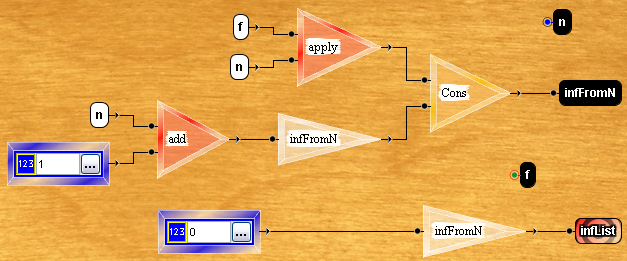
\includegraphics[scale=0.4]{Figures/gcInfList}} \quad
    \subfloat[Using the InfList() Gem To Generate Fibonacci Numbers]{\label{fig:gcInfList-b}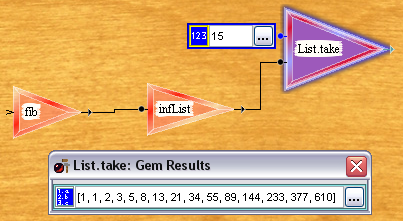
\includegraphics[scale=0.4]{Figures/gcInfListRun}}
  \end{center}
  \caption{Using The InfList() Gem}
  \label{fig:gcInfList}
\end{figure}

\subsubsection{Remedies, Workarounds, And Trade-offs}

The support for Progressive Evaluation in the Gem Cutter is quite strong.  The infinite list issue is relatively minor, only requiring one to create a new subexpression that makes use of the gem which generates the infinite list.  Perhaps a small improvement would be if the user tries to run a gem which generates an infinite list directly, to have the Gem Cutter display the evaluated results rather than just a ``out of memory'' error message.

%------------------------------------------------------------------------------------------------

\subsection{Role-Expressiveness}

As described in \sref{cgframeoutline} the dimension of Role Expressiveness tries to evaluate the environment's support for answering the user's question of ``what is this bit for?''.

\subsubsection{Discussion of Dimension}

The Gem Cutter has a number of aspects to support Role Expressiveness.  For example, all gems have meaningful identifiers attached to them (the name of the function, etc).  Modularity is supported through the use of modules and gems (functions), though while all gems from the standard libraries are organized into modules, all user-created gems go into the same module (the ``GemCutterSaveModule'' module) and creating new modules to use in the Gem Cutter is a nontrivial task (as mentioned in \sref{sec:gemCutterShortcomings}).  In terms of code ``beacons'', we found the same structures identified by Kelso in the VFPE, though rotated 90 degrees as the Gem Cutter arranges items from left to right as opposed to top down (as in the VFPE).  For example, compositional pipelines took the form of a ``vertical string of beads''\cite{Kelso02} in the VFPE, where in the Gem Cutter they became a horizontal string of Gems, etc.  In some ways, list processing created a ``staircase'' of gems, as most of the standard list processing gems (\code{map()}, \code{filter()}, \code{zip()}, etc) have two inputs, the top being a function and the bottom being a list.  A common programming idiom in the functional world is to have the output of list processing functions fed into other list processing functions, which in the case of Gem Cutter results in this left to right, rising ``staircase'' of gems.

\subsubsection{Remedies, Workarounds, And Trade-offs}

The only additional support needed for modularity in regards to the Gem Cutter is the ability for one to more easily create their own modules.  As it stands, one has to resort to writing CAL code by hand, then modifying the Gem Cutter environment to import the modules into the current workspace.

%------------------------------------------------------------------------------------------------

\subsection{Secondary Notation}

As described in \sref{cgframeoutline} the dimension of Secondary Notation explores what support the environment has for conveying extra information to users beyond the official syntax of a notation.

\subsubsection{Discussion of Dimension}

Layout in the Gem Cutter is freeform, and as such can be used to convey meaning to users.  This is very much like Prograph where layout was also freeform, and unlike the VFPE where layout was completely controlled by the environment.  Colour and visual cues are used to convey extra meaning, function gems are coloured red, user-created local functions are coloured a yellow colour, record selection gems a violet colour, and collector gems are black, and emitters are coloured white.  As well, the target gem that represents the gem's return value is coloured as a ``bullseye'' to convey the meaning that it is the overall ``target'' of the current gem.

Commenting is supported through the properties window of any collector gem or the target gem.  The Properties window for the \code{rocket1()} gem described in \sref{sec:eval:diffuseness} is shown in \fref{gcRocketProps}.  In the properties window one can describe and annotate various aspects of the gem in question.  As mentioned the same set of documentation can be done for any collector gem within a gem, thus allowing the ability to comment groups of gems.  However, individual gems other than collector gems cannot be annotated with comments.  In the case of value gems it is possible to ``name'' them by feeding a value gem into a collector gem and then naming the collector gem, however this increases the number of graphic entities on screen thereby negatively impacting Diffuseness.  Additionally, though comments are supported through the properties window of a gem, like the VFPE there is no visual cue that such a comment exists.

\insertFigure{4.5}{gcRocketProps}{The \code{rocket1()} Gem's Properties Window}

\subsubsection{Remedies, Workarounds, And Trade-offs}

The main remedy to problems associated with Secondary Notation that Green describes is to ``provide tools in the system to allow components to be labeled and described and their relationships made explicit'' \cite{green98}.  The Gem Cutter does this to a certain degree with the Properties window, but it is very coarse grained -- there is not enough support in the form of tools to allow sub-parts of gems to be documented and described.

It is also worth noting that Secondary Notation often trades off against Viscosity, as if the structure is changed, then the secondary notation becomes obsolete and also needs to be changed.  In the case of the Gem Cutter when the arguments and return types of a gem change, the properties are automatically updated, which helps to mitigate this concern.  Specifically, if arguments are removed from the gem definition, then they are also automatically removed from the properties window.  If arguments are added then an entry for the argument will be added automatically to the properties of the gem, however a meaningful description still needs to manually be added by the user.  Other metadata stored in the properties window such as author name, description of the gem, etc, will also have to be maintained manually by the user.

%------------------------------------------------------------------------------------------------

\subsection{Viscosity}

As described in \sref{cgframeoutline} the dimension of Viscosity tries to measure an environment's resistance to change.

\subsubsection{Discussion of Dimension}

The biggest issue in terms of Viscosity in the Gem Cutter is the type dependency issue between gems described in \sref{sec:gemCutterShortcomings}.  This imposes a serious impediment on a user to refactor existing gem designs.

The manual layout problem described by Kelso in \cite{Kelso02} is somewhat mitigated by the ability in Gem Cutter to instruct the environment to automatically rearrange all items on the tabletop\footnote{Via the ``Tidy Tabletop'' menu command}.  There is still overhead associated with making changes to expressions due to the having to make and break connections between gems, and move them around to make room for whatever changes need to be made.  This became particularly evident while performing the ``straw-test'' of making the small change to account for air resistance to the rocket trajectory problem, as a significant time consuming aspect of the change in the Gem Cutter version of this problem was breaking the connection between the calculation of the new horizontal and vertical velocities and the collector gem which collected these values, and inserting the gems to incorporate the change to air resistance.  In terms of time taken, incorporating the air resistance change into the Gem Cutter version of the problem was done three times, each application of the change was timed, and took 172 seconds on average to complete.  This is dramatically better than the LabVIEW (508.3 seconds) and somewhat better than the Prograph (193.6 seconds) results, but worse than the VFPE (105 seconds).

One thing worth noting is that the change for air resistance was confined only to the \code{rocket1()} gem, and not the \code{rocketTester()} gem.  Thus the type dependency issue was not encountered in this test.  If \code{rocketTester()} did have to be changed due to the changes in \code{rocket1()} the amount of time taken likely would have been dramatically higher.

\subsubsection{Remedies, Workarounds, And Trade-offs}

Green notes than an important point to consider about Viscosity is that it is not always harmful \cite{green98}.  High viscosity may encourage users to reflect more about the problem before ``diving in'' (though this would be an example of negatively impacting Premature Commitment).  Low Viscosity may encourage users to make changes more often than need be, and as a result increase the Error-Proneness of the system.

The main workaround for extremely viscous environments is to detach from the environment itself.  That is, to use a different environment with very low viscosity to plan out a solution to the problem, then to translate the solution in the low viscosity environment to the high viscosity environment.  For example, one may use pen and paper to sketch out a gem design, changing as problems are encountered, and then recreate the design in Gem Cutter.  This negatively impacts Premature Evaluation as one cannot ``execute'' a drawing on paper.  Alternatively, a possible workaround used at times by the author of this thesis was to write a solution in a textual language that was less viscous, and then translate that text-based solution to the Gem Cutter.  However, this would seem counterintuitive to the motivation behind using the Gem Cutter in the first place.

With respect to the rearranging the layout problem, a possible workaround is to heavily decompose the problem into very small functions.  Making a change to the internal structure of a gem is easy when the gem is small.  Counterbalancing this is the type dependency issue -- if another gem depends on the one being worked on then changing the type signature of the function is problematic, and the more gems there are, the greater the likelihood there will be a type dependency issue between them.

%------------------------------------------------------------------------------------------------

\subsection{Visibility}

As described in \sref{cgframeoutline} the dimension of Visibility is concerned with the environments support for making required materials easily accessible.

\subsubsection{Discussion of Dimension}

In terms of Visibility, navigational visibility is generally strong in the Gem Cutter, as the number of actions needed to find a particular gem in a gem design is usually very small, at most being a simple scrolling of the window to find what one is looking for.  If a gem's design becomes overly ``messy'' or ``cluttered'', a user can select the ``Tidy Tabletop'' option on the view menu to have the environment automatically arrange gem groupings in a top-down manner.  Alternatively, the Scope Window in the top left corner (seen in \fref{gcScopeWindow}) of the Gem Cutter interface, gives a hierarchical, tree-like listing of all components currently on the tabletop.  Clicking any item in this list will immediately center the tabletop on that item.  So in the worst case finding any item in a gem design is a matter of one or two clicks.  Note that as well, any subexpression in the Scope Window can be collapsed to allow one to focus on other parts of the gem design.  In \fref{gcScopeWindow} is seen with the ``hdist'', ``hveloc'', and ``mass'' collector gem expressions being collapsed, and all others being expanded.  

\insertFigure{2}{gcScopeWindow}{The Scope Window For The \code{rocket1()} Gem}

Predefined functions from the standard libraries are organized into modules, and are easy to find via the Gem Browser.  As well, as mentioned in \sref{sec:gemCutterUsefulApps} the Gem Browser also allows one to do a textual search for gems with particular names, input types, return types, or number of arguments.

A significant problem related to Juxtaposability in that at any given time only a single gem design can be open.  This makes working on multiple gems at the same time artificially difficult, as to open up another gem's design one has to save the current gem, then open the design of the other gem.

\subsubsection{Remedies, Workarounds, And Trade-offs}

The obvious solution to the juxtaposibility problem would be to allow multiple gems to be open at once.  Since the tabletop is a sub-window of the main Gem Cutter window, it would seem that there is no reason why this cannot take place as it would just mean allowing a second sub-window to be open.  This would allow one to switch back and forth between multiple gem designs easily.  However, given the fact that gem designs often take up a considerable amount of screen space, even if multiple gems could be open at the same time, it might be difficult or impossible to view them side-by-side.  Short of being able to ``zoom-out'' on a gem design to make it take less space (which would make seeing the individual components more difficult) it would seem that there is no solution to this problem.

As it stands, the only workaround for users to the juxtaposibility problem is to take a screenshot of a gem's design from a separate program, and then refer back to the screenshot as needed\footnote{This is what was done when doing the viscosity ``straw-test'' of making the small change to the rocket trajectory program}.  A significant limitation of this is that it is not uncommon for gem designs to scroll off the screen, making taking a screenshot of an entire gem's design difficult or impossible.

\begin{comment}

\section{Outline Of An Experiment For Evaluating The Effectiveness Of The Gem Cutter}

In the preceding section we explored a qualitative evaluation of the Gem Cutter with a bias toward a pedagogical viewpoint.  However, a useful compliment to this would be to explore a more \emph{quantitative} evaluation of the environment.  In this section we will outline an experiment which could provide a meaningful empirical evaluation of the Gem Cutter.

\subsection{Avenues of Evaluation}

\cite{Kelso02} outlined an experiment for his VFPE in which he outlined two possible avenues of for empirical evaluation of the VFPE:

\begin{enumerate}
	\item Evaluating the general adequacy of the environment
	\item Investigating Visual Programming proper
\end{enumerate}

The first is focused on conducting experiments to evaluate the general adequacy of the programming environment.  Such experiments would focus on showing quantitatively that for programmers experienced with textual languages, that the visual environment is not significantly worse than the textual alternative.  That is, that the environment is ``feature-equivalent'' to a given textual environment.

The second is for the purpose of exploring the textual/visual division.  That is, experiments designed here would be for the purpose of identifying differences that are due solely to the respective modes of display and the programming environment tools.  This was the type of experiment that Kelso outlined for his VFPE.  This requires a textual environment which is roughly equivalent to the VFPE.  
Given that the VFPE from a semantics and abstract syntax viewpoint is very similar to Haskell, Kelso believed that an experiment comparing the two would reveal differences between the visual and textual forms of representation.  Given that the Gem Cutter truly is the visual representation of CAL code, it would seem that an experiment of this form with the Gem Cutter and CAL would be more telling of the differences between the visual and the textual.

In addition to these, we can foresee other avenues for empirical evaluation of the Gem Cutter, most notably that of functional versus object-orientated programming.  There have already been studies which have explored the differences between the two paradigms (FIXME - references??), but they have largely been based solely in the textual world.  Similar experiments using the Gem Cutter (a visual environment rooted in the functional paradigm) and one of the common object-orientated environments (such as Prograph, Alice, or Scratch) would be an interesting addition to the work exploring the difference between the two paradigms.

For our purposes as educators however, we are more interested about how effective the Gem Cutter can be as a learning tool for students.  As such, we shall identify an experiment which explores two other avenues of exploration.  The first is to assess if the Gem Cutter can meet a typical set of learning objectives (ie - ``Does the student learn the concept?''), and the second assesses the transfer of skill to another environment (ie - ``Can the student apply what he/she learned to a different language?'').

\subsection{Difficulties}

Assessing which of two competing methods of instruction is more effective seems at first glance to be a simple task.  Simply teach one subject with both methods and compare the results of the two approaches.  However, as outlined by McKeachie in \cite{teachingTips} there are some difficulties or ``hidden traps'' that arise in trying to evaluate two different approaches to instruction.

The first category of problems are methodological, 

From Teaching Tips, \cite{teachingTips}:

methodological problems:

\begin{itemize}
	\item Hawthorne effect - instructor enthusiasm can influence quality of instruction, students react differently when they know they are being taught by an experimental method -- necessitates evaluation over period of time
	\item Finding control group -- different classes have different makeups of students, some instructors are better than others (so if method is successful how much is the method and how much the instructor)
\end{itemize}

criterion problem - you want to ``know what each group learned that the other did not.  Thus a comparison of the lecture method with a discussion method based on a common final examination from a textbook does not really compare what the two groups of students learned in their different classes, but rather what they learned from reading the text.''  ''criterion measure should sample progress on \textit{all} goals, not just a small sample chosen for a particular method.''  Student motivation -- students are motivated to get good grades, and thus may compensate for poor instruction, thereby obfuscating research results.

\subsection{Preparation}


\subsection{Group Selection}


\subsection{Measurement}

\section{Misc Notes}

\cite{Bayliss09} in 3.7 talks about important points in assessing the use of games, which may be relevant to this experiment.

\end{comment}